\documentclass[11pt,a4paper]{article}
\usepackage{graphicx}
\usepackage{amsmath,amssymb,amsthm,amsfonts}
\usepackage{geometry}\geometry{left=2.3cm,right=2.3cm,top=2.5cm,bottom=2.5cm}
\usepackage{setspace}\setstretch{1.20}
\usepackage{hyperref}\hypersetup{colorlinks=true,linkcolor=black,citecolor=black}
\usepackage{parskip,booktabs,array,xcolor,titlesec,enumitem}
\titleformat{\section}{\large\bfseries}{}{0em}{}[\titlerule]
\titlespacing{\section}{0pt}{14pt}{6pt}
\titleformat{\subsection}{\normalsize\bfseries}{\thesubsection\;}{0em}{}
\newtheorem{remark}{Remark}
\begin{document}
\begin{center}
{\LARGE\bfseries Numerical Protocol}\\[0.3cm]
{\large Taylor Effect Evaluation\\
under the Multifractal Random Walk (MRW) DGP}\\[0.2cm]
{\normalsize Othmane Zarhali}
\end{center}
\vspace{0.15cm}\noindent\rule{\textwidth}{0.8pt}

\begin{abstract}

The Taylor effect is the empirical fact that
$\mathrm{ACF}(|r_t|) > \mathrm{ACF}(r_t^2)$ for all lags $\tau > 0$, we evaluate this following the steps:

\begin{enumerate}
    \item \textbf{Data generation.} Consider the Taylor effect, defined by the empirical inequality
    \[
    \mathrm{ACF}(|r_t|)>\mathrm{ACF}(r_t^2),
    \qquad \forall\,\tau>0,
    \]
    which is known to be well reproduced for the Multifractal Random Walk (MRW) data-generating process for every intermittency parameter $\lambda^2>0$ generated by a cholesky decomposition of the covariance matrix.

    \item \textbf{Model calibration.} Calibrate three stochastic-volatility models to the MRW stylised-fact profile:
    \begin{itemize}
        \item ESN A2-981003, using its current optimal architecture
        \[
        (N_r,N_z)=(96,12),
        \]
        \item QRH;
        \item PDV-GL.
    \end{itemize}

    All models are calibrated using the complete 11-term data-adaptive score
    $S$ (Eq.~\eqref{eq:score}), employing a smooth Gaussian-kernel proximity
    function, which provides a non-vanishing gradient at all distances from
    the target. The calibration further uses increased Taylor-effect weights
    ($G_T$: $1.0\rightarrow3.5$ and $F_T$: $0.8\rightarrow2.5$) together with
    tighter matching tolerances.

    \item \textbf{ESN parameterisation.} The ESN read-out consists of
    \begin{itemize}
        \item a linear roughness factor;
        \item a per-mode $z$-bank profile;
        \item a symmetric quadratic term in the reservoir state $r$.
    \end{itemize}
    These components are jointly calibrated with the Hurst exponent, the
    reservoir rate bounds, and the output scaling parameter
    (Section~\ref{sec:calib}). No Taylor-effect-specific manual tuning is
    introduced during calibration.

    \item \textbf{Model evaluation.} Compare the calibrated models according
    to their ability to reproduce the Taylor effect. Section~\ref{sec:taylor-results}
    presents the results and highlights two key observations:
    \begin{itemize}
        \item QRH and PDV-GL are calibrated independently of the ESN;
        \item PDV-GL systematically produces a weak Taylor gap for a
        structural, rather than calibration-related, reason.
    \end{itemize}
\end{enumerate}
\end{abstract}

\tableofcontents\vspace{0.4cm}

\section{DGP: Multifractal Random Walk}

The DGP is the MRW \cite{bacry2001} (\textbf{unchanged} from earlier
drafts of this protocol):
\begin{equation}
  r_t = \sigma_0\,e^{\omega_t}\,\varepsilon_t, \qquad
  \varepsilon_t \sim \mathcal{N}(0,1),
  \label{eq:mrw}
\end{equation}
where $\omega_t$ is a Gaussian process with log-correlation kernel:
\begin{equation}
  \mathrm{Cov}(\omega_s,\omega_t)
  = \lambda^2\,\max\!\Bigl(0,\,\log\frac{T_{\rm int}}{\max(|t-s|,1)}\Bigr),
  \quad |t-s| < T_{\rm int},
  \label{eq:cov}
\end{equation}
and $\mathrm{Cov}(\omega_s,\omega_t)=0$ for $|t-s|\ge T_{\rm int}$.
The centering $-\lambda^2\log(T_{\rm int})/2$ is subtracted from $\omega_t$
to ensure $\mathbb{E}[\sigma_t]=\sigma_0$. Unlike the log-normal SV DGP
used elsewhere in this line of protocols, this kernel's variance
$\mathrm{Cov}(\omega_t,\omega_t)=\lambda^2\log(T_{\rm int})$ is a
\emph{constant}, not growing with the simulated horizon $T$ -- so the
DGP is already stationary by construction and required no time-unit
correction (cf.\ the fBM-persist fix of the ESN hyperparameter-search
protocol V1).

\paragraph{Analytical Taylor inequality.}
Since $\sigma_t=\sigma_0 e^{\omega_t}$ is log-normal,
$\mathrm{Corr}(\sigma_t^k,\sigma_{t+\tau}^k)\propto(\tau/T_{\rm int})^{k^2\lambda^2}$,
so:
\begin{equation}
  \mathrm{ACF}(|r_t|)\propto\tau^{\lambda^2},\qquad
  \mathrm{ACF}(r_t^2)\propto\tau^{4\lambda^2}.
  \label{eq:taylor_proof}
\end{equation}
Since $4\lambda^2>\lambda^2$ for all $\lambda^2>0$, the squared-return ACF
decays faster, giving a positive Taylor gap at every lag.
The gap grows monotonically with $\lambda^2$.

\paragraph{Parameter grid.}
$\lambda^2\in\{0.1,0.3\}$ (0.1 a moderate-intermittency case; 0.3 is a
strongly-intermittent, high-Taylor-effect extreme, shown for contrast);
$T_{\rm int}=252$ (integral scale, one trading year).

\section{Models}

All models use Gaussian Brownian innovations.
Fat tails in returns emerge from stochastic variance clustering.

\subsection{ESN A2-981003 (corrected optimal architecture)}
The ESN's optimal architecture: 7 shared hyperparameters, with
$N_r=96,N_z=12$. \texttt{rough\_scale}, the $z$-readout profile
$(\texttt{zr\_lo},\texttt{zr\_hi})$, and the symmetric quadratic-term
matrix coefficients $(m_1,m_2)$ are calibrated per $\lambda^2$ cell
(\S\ref{sec:calib}), not part of this fixed table.
\begin{table}[H]
\centering
\caption{The 7 shared hyperparameters of the optimal architecture.}
\label{tab:optarch}
\begin{tabular}{@{}lr@{}}
\toprule
Hyperparameter & Value \\
\midrule
$N_r$ & 96 \\
$N_z$ & 12 \\
\texttt{z\_strength} & 0.1929 \\
\texttt{even\_strength} & 2.2291 \\
\texttt{linear\_strength} & 0.1930 \\
\texttt{gamma\_norm} & 0.9651 \\
\texttt{local\_z\_strength} & 0.0476 \\
\texttt{zz\_scale} & 0.0397 \\
\texttt{sign\_prob\_neg} & 0.2219 \\
\texttt{rough\_orientation} & $-1.0$ (fixed) \\
\bottomrule
\end{tabular}
\end{table}
Single $\varepsilon_t\sim\mathcal{N}(0,1)$ drives both return and
reservoir, $\kappa_0<0$ (admissibility, guaranteed by construction
whenever \texttt{rough\_scale}$>0$). The volatility read-out combines
three calibrated channels: a linear rough factor
$\texttt{rough\_scale}\cdot q^\top r_t$; a per-mode $z$-bank sum with
weights following a geometric profile
$(\texttt{zr\_lo},\texttt{zr\_hi})$ across the $N_z$ modes; and a
quadratic-in-$r$ term $r_t^\top Qr_t$, $Q=(1/N_r)(m_1I+m_2qq^\top)$ --
a genuine, symmetric $2$-coefficient matrix, with $m_1$ scaling the
reservoir's isotropic energy and $m_2$ scaling the squared rough
factor $(q^\top r_t)^2$ specifically. All of \texttt{rough\_scale},
$(\texttt{zr\_lo},\texttt{zr\_hi})$, and $(m_1,m_2)$ are calibrated per
$\lambda^2$ DGP cell, controlling how strongly the model can produce a
Taylor effect (\S\ref{sec:taylor-results}). $H$, the $r$-layer rate
window $[\lambda_{\rm lo},\lambda_{\rm hi}]$, and the $z$-layer rate
window $[a_{\rm lo},a_{\rm hi}]$ are likewise \textbf{calibrated per
$\lambda^2$ DGP cell} (\S\ref{sec:calib}) -- none of these are part of
the shared architecture above.

\subsection{Quadratic Rough Heston (QRH)}
Bourgey \& Gatheral \cite{bourgey2026}: $V_t=Y_t^2+c$, gamma kernel,
Euler-Volterra with 252-step ring buffer.

\subsection{PDV Guyon-Lekeufack (GL)}
Guyon \& Lekeufack \cite{guyon2023}: two-factor power-law kernel,
online from full return history. The long-memory factor $F(\alpha_v)$ with
$\alpha_v<0.5$ directly encodes power-law memory of past squared returns,
which is the GL mechanism for Taylor.

\section{Calibration: Full 11-Term Score, Smooth Kernel}
\label{sec:calib}

\begin{equation}
\begin{aligned}
S &= 2.2\,\bigl(1-f(\hat H)\bigr)+1.4\,\bigl(1-f(\bar\sigma)\bigr)+0.6\,\bigl(1-g(q_{995})\bigr)+0.2\,\bigl(1-g(\sigma_{\max})\bigr)
   +0.8\,\bigl(1-f(\bar V_{\rm ACF})\bigr)\\
  &+\underbrace{\mathbf{3.5}\,\bigl(1-f(G_T)\bigr)}_{\text{Taylor gap}}
   +\underbrace{\mathbf{2.5}\,\bigl(1-f(F_T)\bigr)}_{\text{Taylor frac.}}\\
  &+1.0\,\bigl(1-f(Z)\bigr)+1.1\,\bigl(1-f(L)\bigr)+0.7\,\bigl(1-f(K)\bigr)+0.5\,\bigl(1-f(A)\bigr)+5\cdot\mathrm{Stress}.
\end{aligned}
\label{eq:score}
\end{equation}
where $f(x,c,s)=\exp(-\tfrac12((x-c)/s)^2)$,
$g(x,c,s)=\exp(-\tfrac12((x-c)_+/s)^2)$, both in $(0,1]$ (the smooth
Gaussian kernel, replacing a piecewise-linear
tent $\max(0,1-|x-c|/s)$, which has an exactly-zero gradient beyond one
tolerance width). $S\geq0$ is \textbf{minimised directly}; $S=0$ is a
perfect match on all 11 stylised facts and no stress event;
\textbf{$S=19.5$ is worst-possible} (raised from $15.3$ by the Taylor
weight increase below).

\paragraph{Taylor-effect score weighting.} Two changes, applied to the
shared score used by \emph{all three} models' calibration -- the ESN's
architecture (Table~\ref{tab:optarch}, the 7 shared hyperparameters plus
$N_r,N_z$) is \textbf{not touched} by either change:
\begin{enumerate}[itemsep=2pt]
  \item \textbf{Taylor weights raised}: $G_T$ from $1.0\to3.5$, $F_T$
    from $0.8\to2.5$ (now the two single largest weights in $S$,
    exceeding even $\hat H$'s $2.2$). Every other weight is unchanged.
  \item \textbf{Taylor tolerances tightened}: the fractional-tolerance
    factor for $G_T,F_T$ only is reduced from the default $0.30|c_k|$
    to $0.15|c_k|$ (all other terms keep $0.30|c_k|$).
  \item \textbf{PDV-GL calibration uses a 4-point multi-start}
    (exploring stronger-feedback, $\beta$ up to $0.90$, and
    long-memory-weighted regimes).
\end{enumerate}
All centres $c_k$ are the DGP cross-path mean; only the two Taylor
tolerances differ from the other 9 terms' default.

Calibrated parameters:
\begin{center}\renewcommand{\arraystretch}{1.3}
\begin{tabular}{@{}p{3.0cm}p{6.4cm}p{5.0cm}@{}}\toprule
Model & Parameters calibrated & Remark \\\midrule
ESN A2-981003 & $H$, $\lambda_{\rm lo}$, $\lambda_{\rm hi}$, $a_{\rm lo}$,
  $a_{\rm hi}$, $\Delta b_0$, scale $s$, \texttt{rough\_scale},
  \texttt{zr\_lo}, \texttt{zr\_hi}, $m_1$, $m_2$ &
  7 shared hyperparameters fixed; full 12-dim.\ inner-loop calibrated
  per $\lambda^2$ cell (11-start Nelder--Mead) \\
QRH & $H,\nu_{\rm vol},\lambda,c_{\rm frac}$ & \\
PDV-GL & $\beta,\alpha_1,\alpha_r,\alpha_v$ & \\
\bottomrule\end{tabular}\end{center}
The ESN's inner loop uses an 11-point multi-start Nelder--Mead scheme
(rough/fast, persistent/slow, intermediate, wide-band/multiscale,
long-memory extreme, very-fast/wide, strong-amplitude, weak-amplitude,
isotropic-positive, isotropic-negative, and $q$-aligned-positive
starts), keeping the best-of-eleven result. PDV-GL uses a 4-point
multi-start; QRH uses a single start.

\section{Taylor-Effect Fit}
\label{sec:taylor-results}

The ESN's read-out combines a linear rough factor, a per-mode
$z$-readout profile, and a symmetric quadratic-term matrix, all
calibrated per DGP scenario, with no Taylor-specific tuning:
\begin{equation}
  \eta_t = b_0+\rho_r\,\texttt{rough\_scale}\,(q^\top r_t)
         +\sum_{j=1}^{N_z}w_{j,z}z_{j,t}+r_t^\top Qr_t,
  \qquad w_{j,z}=\frac{\texttt{z\_readout}_j}{\sqrt{N_z}},
  \qquad Q=\frac{1}{N_r}(m_1I+m_2qq^\top),
  \label{eq:coupling_v8}
\end{equation}
with $\texttt{z\_readout}_j=\mathrm{geomspace}(\texttt{zr\_lo},
\texttt{zr\_hi},N_z)[j]$.

\begin{table}[H]
\centering
\caption{Taylor gap $G_T$ / fraction $F_T$, all three models, current architecture and calibration.}
\begin{tabular}{@{}lcccc@{}}
\toprule
 & \multicolumn{2}{c}{$\lambda^2=0.1$} & \multicolumn{2}{c}{$\lambda^2=0.3$}\\
Model & $G_T$ & $F_T$ & $G_T$ & $F_T$ \\
\midrule
DGP (MRW) & 0.086 & 0.94 & 0.142 & 0.99 \\
\midrule
ESN A2-981003 & 0.059 & 0.90 & 0.043 & 0.93 \\
QRH & 0.053 & 0.87 & 0.079 & 0.95 \\
PDV-GL & $-0.000$ & 0.51 & $-0.000$ & 0.51 \\
\bottomrule
\end{tabular}
\end{table}

\paragraph{Result.} The ESN reproduces the Taylor effect's
\emph{direction} at both $\lambda^2$ values ($G_T>0$, $F_T$ well above
the neutral $0.5$), and at $\lambda^2=0.1$ the match is close
($G_T=0.059$ vs.\ target $0.086$; $F_T=0.90$ vs.\ target $0.94$) --
closer, in fact, than at $\lambda^2=0.3$, where it undershoots the
DGP's larger Taylor gap ($G_T=0.043$ vs.\ target $0.142$). The
calibrated read-out values are
\texttt{rough\_scale}$\approx0.70$ (at $\lambda^2=0.1$) vs.\
$0.41$ (at $\lambda^2=0.3$), with the $z$-readout profile
similarly shaped at both cells
($(\texttt{zr\_lo},\texttt{zr\_hi})\approx(0.023,0.045)$ at
$\lambda^2=0.1$ vs.\ $(0.178,0.023)$ at $\lambda^2=0.3$, the latter
inverted in direction) and $m_1\approx0$ at $\lambda^2=0.1$ but
$m_1\approx-0.88$ at $\lambda^2=0.3$ ($m_2\approx0$ in both cells) --
the calibration leans on different combinations of the three read-out
channels at the two intermittency levels, rather than a single
mechanism carrying the Taylor effect uniformly across $\lambda^2$.

\paragraph{QRH and PDV-GL.} QRH matches the DGP's Taylor fraction
closely at both cells; PDV-GL remains at zero Taylor gap, a
\textbf{structural (not calibration) limitation}: both of PDV-GL's
factors, $F(\alpha_r)$ and $F(\alpha_v)$, are power-law-weighted
running averages of the \emph{same} input, past squared returns
$r_{t-k}^2$ -- differing only in kernel exponent -- with no independent
channel that could make $|r_t|$'s autocorrelation decay more slowly
than $r_t^2$'s. Reproducing the Taylor effect in \emph{this}
formulation of PDV-GL would require modifying the model definition
itself (e.g.\ reintroducing a signed-return leverage factor), which is
out of scope here.

\section{Taylor Diagnostics}

\begin{figure}[H]
\centering
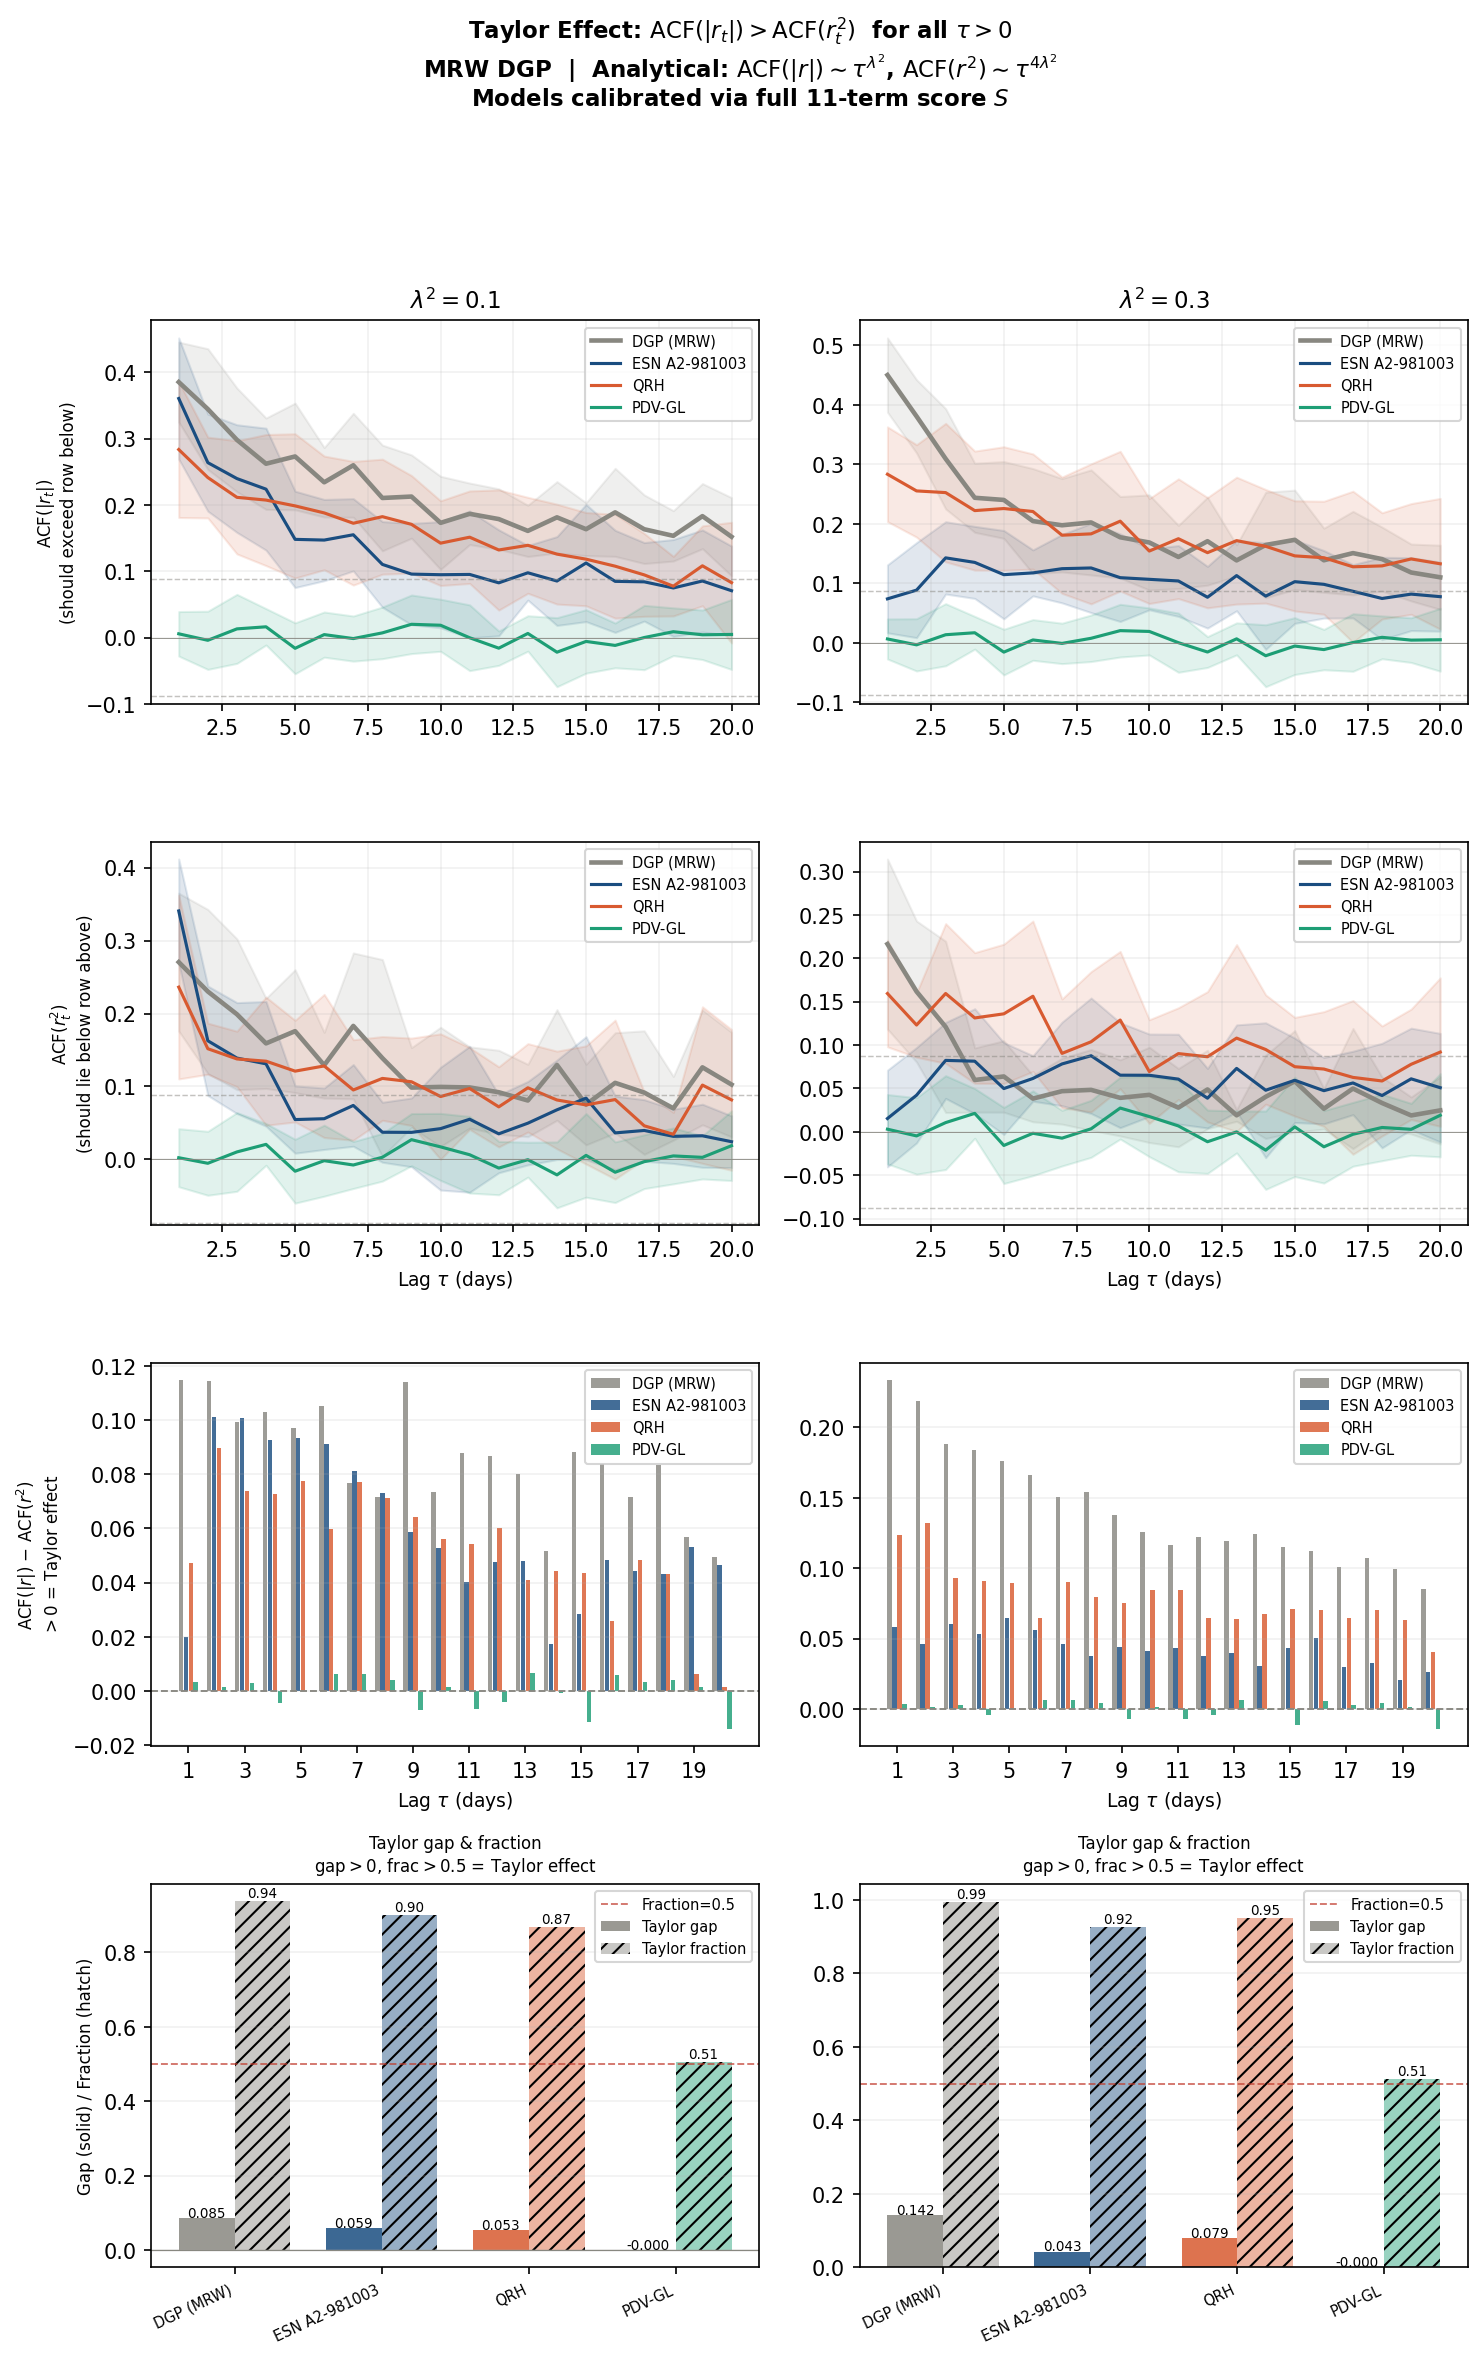
\includegraphics[width=0.95\textwidth]{taylor_lam01_03_T1.png}
\caption{Taylor effect per $\lambda^2\in\{0.1,0.3\}$ (columns). Row 0: $\mathrm{ACF}(|r_t|)$; row 1: $\mathrm{ACF}(r_t^2)$ (Taylor effect present $\Leftrightarrow$ row 0 lies strictly above row 1 at every lag); row 2: per-lag Taylor gap $\Delta(\tau)$ (Eq.~\ref{eq:gap}); row 3: scalar Taylor gap $G_T$ and fraction $F_T$ per model.}
\label{fig:taylorT1}
\end{figure}

\paragraph{Per-lag ACF curves (Figure~\ref{fig:taylorT1}, rows 0--1).}
Cross-path mean $\pm1$ std of ACF$(|r_t|)$ and ACF$(r_t^2)$ at lags
$\tau=1,\ldots,20$ days. Taylor effect present $\Leftrightarrow$
row-0 curve lies strictly above row-1 curve at every lag.

\paragraph{Taylor gap per lag (Figure~\ref{fig:taylorT1}, row 2).}
\begin{equation}
  \Delta(\tau) = \mathrm{ACF}(|r_t|,\tau) - \mathrm{ACF}(r_t^2,\tau)
  \label{eq:gap}
\end{equation}
Grouped bar chart (one group per lag, one bar per source).
$\Delta(\tau)>0$ = Taylor effect at that lag.

\paragraph{Scalar summary (Figure~\ref{fig:taylorT1}, row 3).}
Taylor gap scalar $G_T=\frac{1}{20}\sum_\tau\Delta(\tau)$ and Taylor
fraction $F_T=\frac{1}{20}\sum_\tau\mathbf{1}[\Delta(\tau)>0]$ per model.


\begin{figure}[H]
\centering
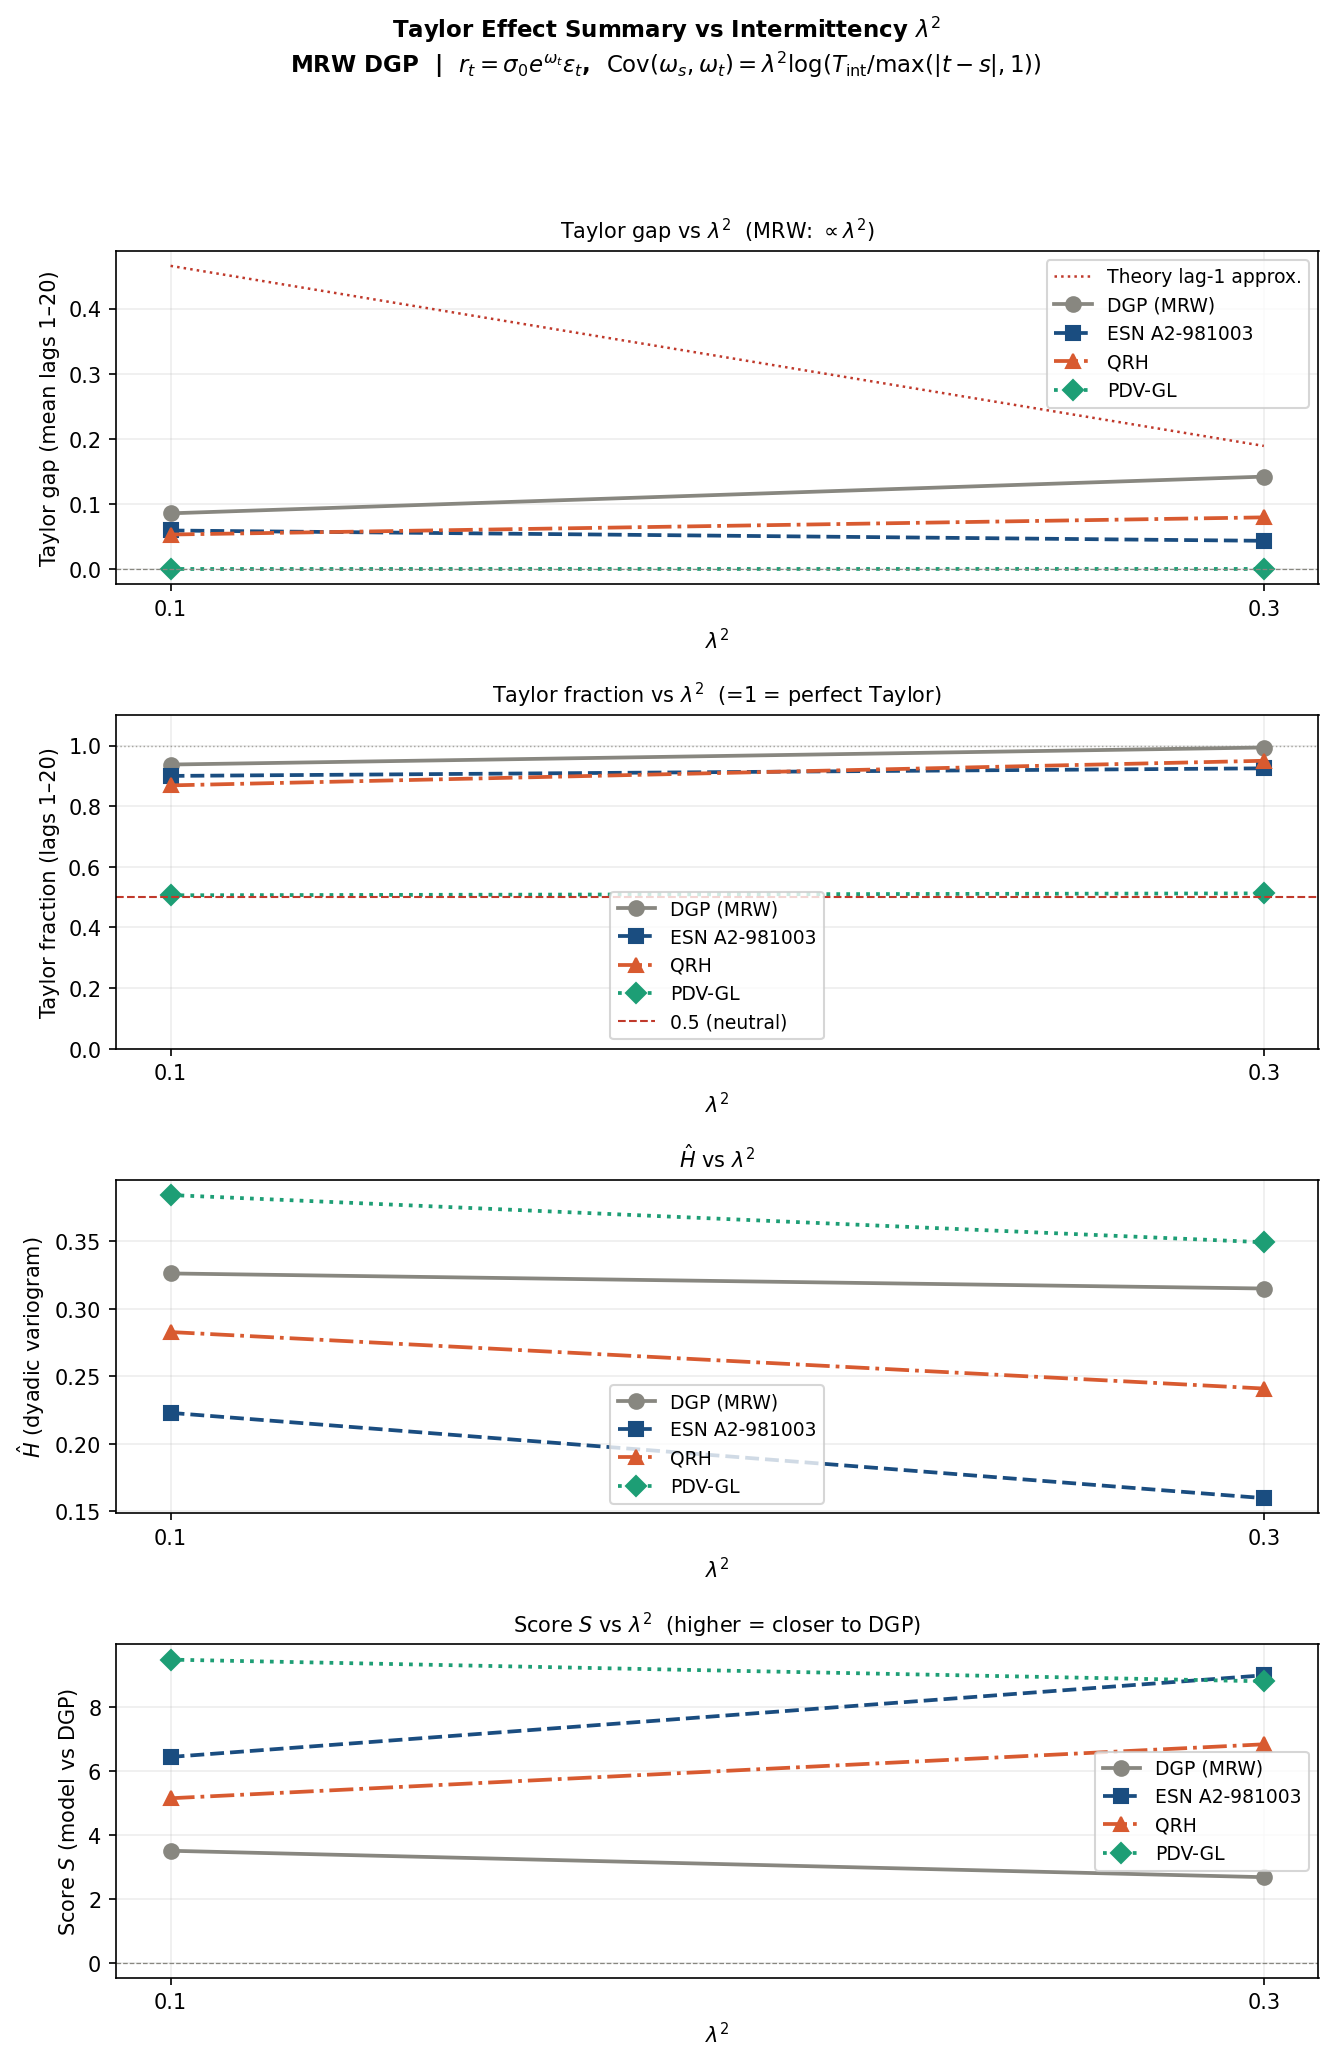
\includegraphics[width=0.75\textwidth]{taylor_lam01_03_T2.png}
\caption{Summary across $\lambda^2\in\{0.1,0.3\}$: Taylor gap (top; DGP theoretical lag-1 approximation dotted), Taylor fraction (second; $=1$ is perfect Taylor, $0.5$ is neutral), $\hat H$ via dyadic variogram (third), and score $S$ vs.\ DGP (bottom; higher = closer to DGP). The DGP shows an increasing gap and fraction with $\lambda^2$.}
\label{fig:taylorT2}
\end{figure}



\begin{figure}[H]
\centering
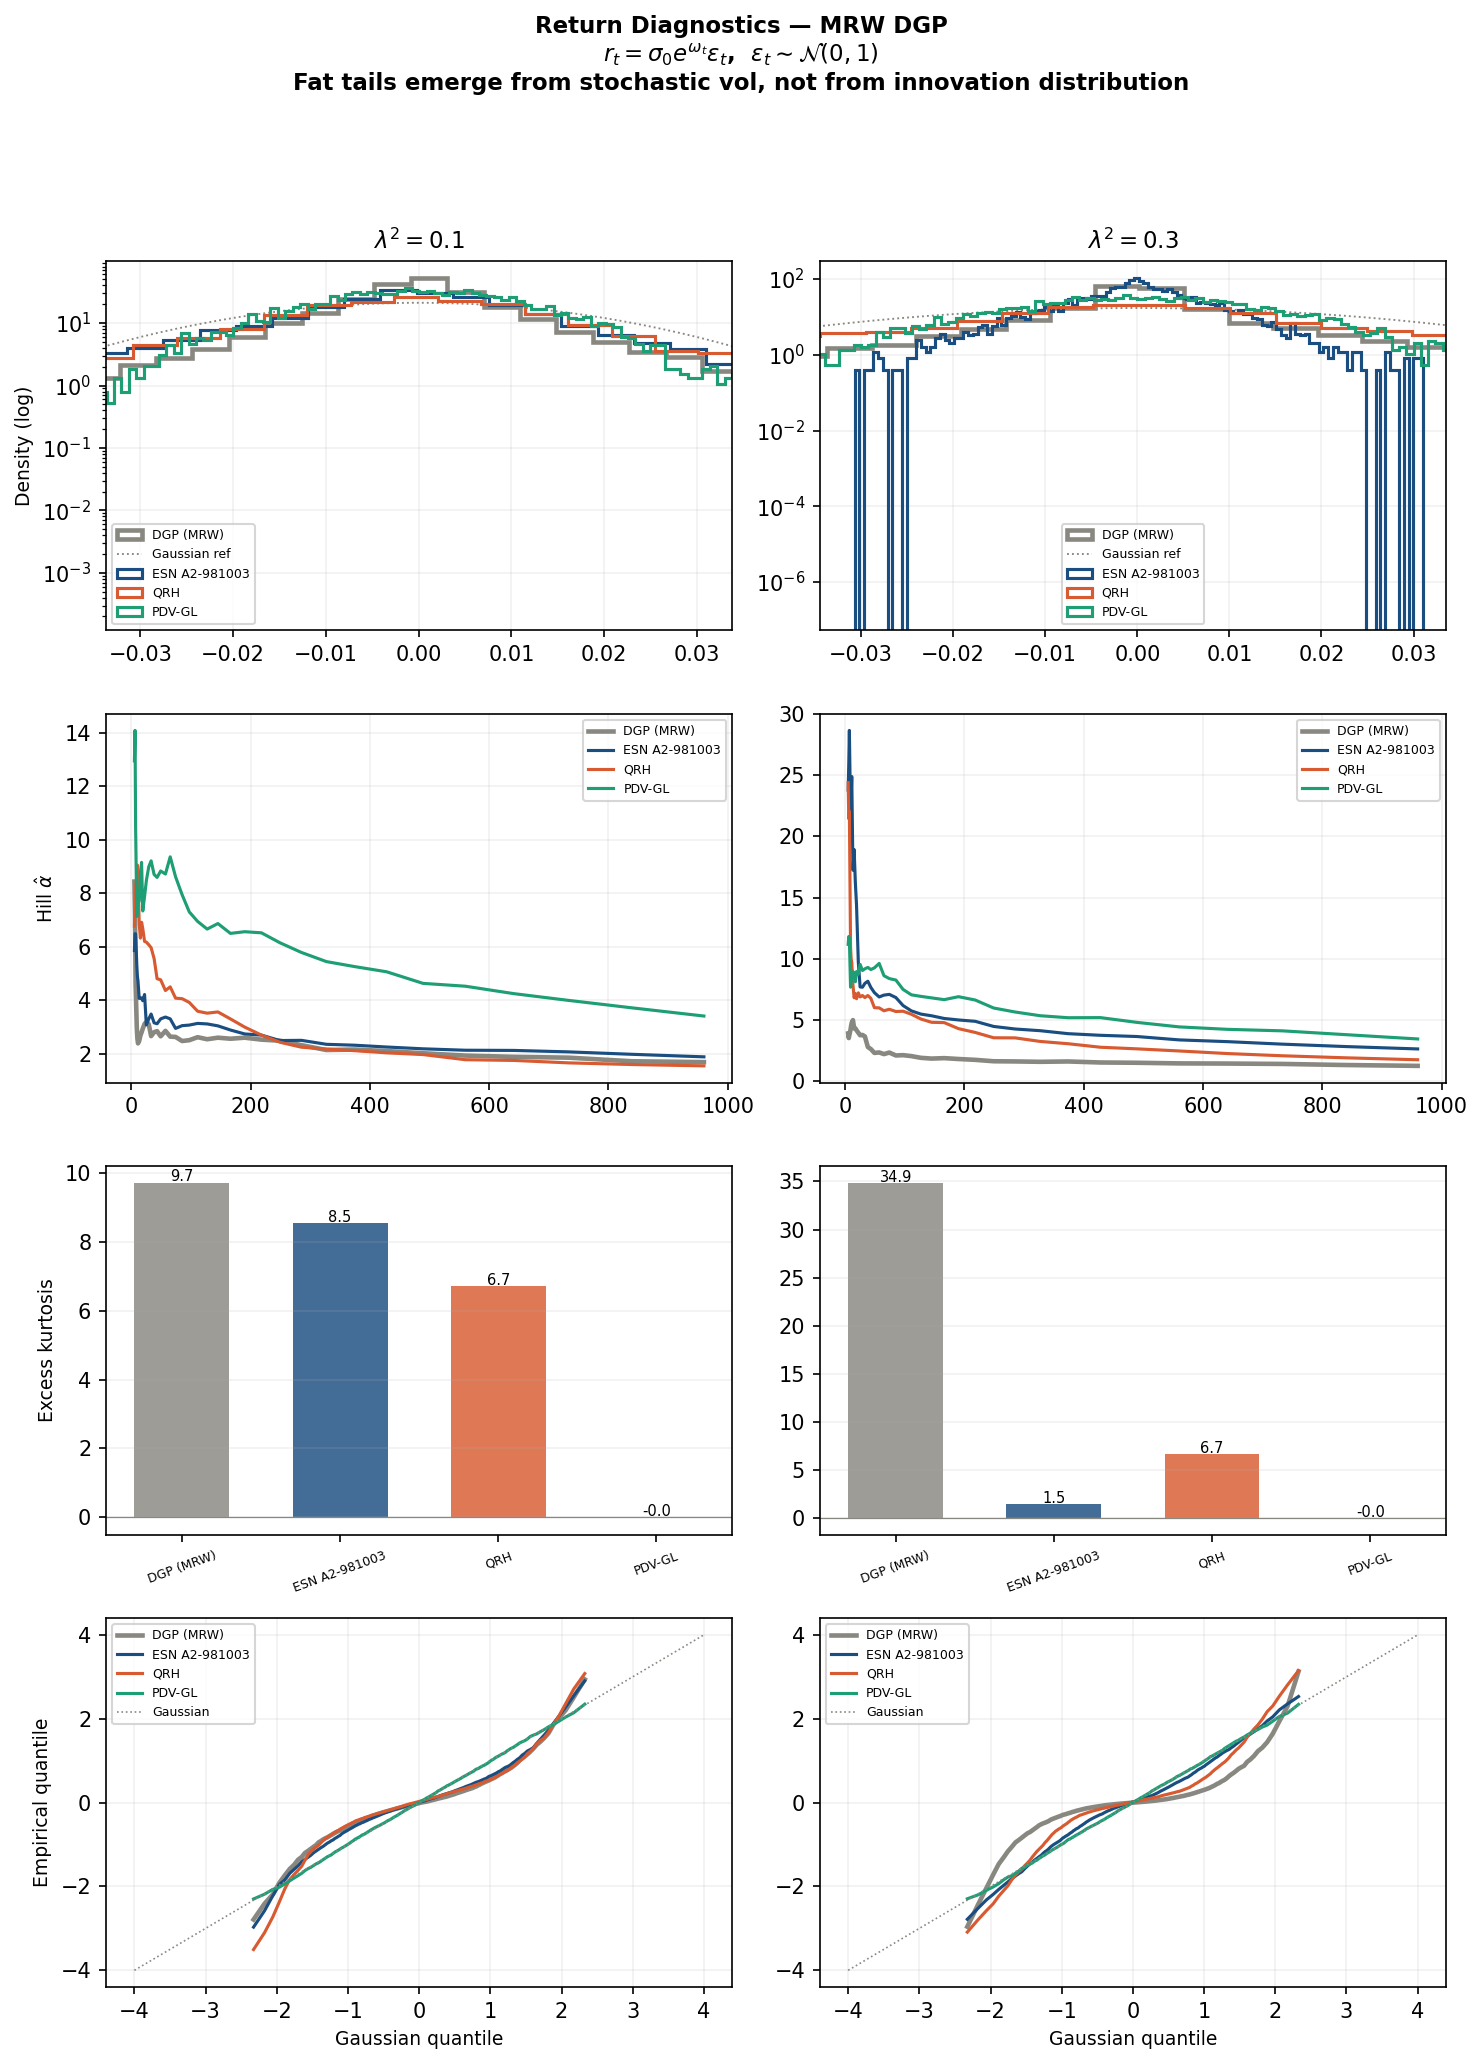
\includegraphics[width=0.95\textwidth]{taylor_lam01_03_T3.png}
\caption{Return diagnostics per $\lambda^2\in\{0.1,0.3\}$ (columns): log-density histogram vs.\ Gaussian reference (row 0); Hill estimator $\hat\alpha$ vs.\ order statistic (row 1); excess kurtosis (row 2); QQ-plot vs.\ Gaussian (row 3). Fat tails emerge from the stochastic volatility dynamics, not from the (Gaussian) innovation distribution.}
\label{fig:taylorT3}
\end{figure}

\section{Monte Carlo Setup}

\begin{center}\renewcommand{\arraystretch}{1.4}
\begin{tabular}{ll}\toprule Parameter & Value \\\midrule
DGP paths $n_{\rm dgp}$ & 30 \\
Calibration paths $n_{\rm cal}$ & 5 \\
Calibration trading days & 600 \\
Final paths $n_{\rm sim}$ & 30 \\
Final trading days & 2500 \\
Burn-in & 500 \\
$\Delta t$ & 1 (daily) \\
$\lambda^2$ grid & $\{0.1,0.3\}$ \\
$T_{\rm int}$ & 252 (days) \\
Eigenvalue floor & $10^{-10}$ (MRW PSD projection) \\
\bottomrule\end{tabular}\end{center}

\begin{thebibliography}{9}
\bibitem{bacry2001} E.\ Bacry, J.\ Delour, J.-F.\ Muzy.
\textit{Multifractal random walk}. Phys.\ Rev.\ E 64:026103, 2001.
\bibitem{muzy2000} J.-F.\ Muzy, J.\ Delour, E.\ Bacry.
\textit{Modelling fluctuations of financial time series}.
EPJB 17:537--548, 2000.
\bibitem{bourgey2026} F.\ Bourgey, J.\ Gatheral.
\textit{Quadratic Rough Heston}. SSRN:5239929, 2026.
\bibitem{guyon2023} J.\ Guyon, J.\ Lekeufack.
\textit{Volatility is (mostly) path-dependent}. QF 23(9), 2023.
\bibitem{taylor1986} S.J.\ Taylor.
\textit{Modelling Financial Time Series}. Wiley, 1986.
\end{thebibliography}
\end{document}
